\section {Desarrollo}
La metodología del presente proyecto se estructuró en diferentes fases para garantizar la correcta implementación del sistema de detección y análisis de vehículos, empleando el modelo YOLO y técnicas avanzadas de visión por computadora. A continuación, se describen cada una de las etapas:

\subsection{Selección del Modelo de Detección de Objetos}

Para este proyecto, se seleccionó el modelo YOLO para la detección de objetos, concretamente de coches. Se ha escogido este algoritmo por su eficacia a la hora de ejecutar su tarea en tiempo real manteniendo una alta precisión en la identificación de objetos.
Específicamente, se utilizó una versión preentrenada del modelo denominada YOLOv11n (yolo11n.pt), ya que está optimizada para su uso en sistemas que requieren analizar velocidad y precisión.  El modelo es capaz de identificar múltiples clases de objetos en un solo pase de red neuronal, pero en este caso solo se quiere reconocer automóviles, entonces se utilizarán las clases [2, 7].

El modelo es conocido por robustez y fácil integración en aplicaciones reales, lo que lo hace adecuado para analizar contextos como el tráfico en tiempo real.
\subsection{Entorno y Datos}

El entorno de trabajo está basado en Python, utilizando bibliotecas especializadas como Ultralytics para trabajar con YOLO y OpenCV para el procesamiento de vídeos.
El dato de entrada es un vídeo de tráfico de coches real.  Este vídeo fue almacenado en un directorio estructurado llamado ../data.  Se creó también una clase personalizada (Video) para extraer información relevante del vídeo como la resolución, los FPS o fotogramas por segundo y la duración total.
El modelo YOLO se cargó desde un directorio preconfigurado.

\subsection{Definición de la Región de Interés (ROI)}
Para simplificar el proyecto y así optimizar los recursos, es preciso centrarse exclusivamente en los objetos que sean interesantes (los coches).  Para ello, se define una ROI dentro de cada frame del vídeo.
Esta región se delimitó mediante coordenadas específicas (x1, y1, x2, y2), que son acordes al área del video donde se esperaba encontrar vehículos en movimiento. La ROI permitió reducir el área que se va analizar y procesar, descartando elementos irrelevantes como el puede ser el cielo o la delimitación del medio de la carretera.

\subsection{Algoritmo de Detección y Seguimiento}
La base de esta práctica ha sido la integración del modelo YOLO con el procesamiento de vídeo. 
Para leer los fotogramas se diseñó un generador de frames a través de la clase Video para así poder iterar sobre cada uno de ellos.  Cada frame es recortado según la ROI antes de ser procesado.
Para detectar los vehículos, se configuró el modelo YOLO para que tan solo se centrara en coches y camiones.  A cada frame se le aplica el método 'track', el cual asigna a cada objeto un identificador único para hacer seguimiento de él a lo largo del tiempo.
Los objetos que se detectan se representan con un cuadro delimitador o bounding box y salen en el vídeo final.


\subsection{Estimación Velocidades}
Una de las partes claves de la práctica fue calcular la velocidad de cada coche utilizando píxeles por frame.  Para ello, se desarrolló lo siguiente:
\begin{enumerate}
    \item Posición del objeto:
    Para cada vehículo que se reconoce, se registraron sus coordenadas de posición en los distintos frames.
    \item Cálculo de Velocidad:
    En base a las diferencias de posición, en píxeles, y el tiempo transcurrido entre los distintos frames (por tasa de FPS), se calcula la velocidad en términos de píxeles por frame.
    Estos valores se imprimen directamente en el vídeo procesado junto con el identificador de cada vehículo.
    \item Visualización:
    Se incluyeron puntos centrales de los vehículos para ilustrar la posición actual y las trayectorias detectadas.
    \item Tráfico:
    Se ha considerado que si se cuentan más de ciertos coches seguidos, entonces se imprimirá en el vídeo que hay tráfico.
\end{enumerate}

\subsection{Visualización de Resultados}
Durante el procesamiento se muestra una ventana emergente que presenta los resultados en tiempo real: la detección de los vehículos, la ROI y las velocidades. Todos los frames procesados se guardan en un archivo de 
salida con OpenCV.  Esto lo que permite es generar un vídeo final para ver en análisis 
resultante de todos los cálculos realizados.
A continuación se ven las distintas secuencias del vídeo:
\begin{figure}[h!]
    \centering
    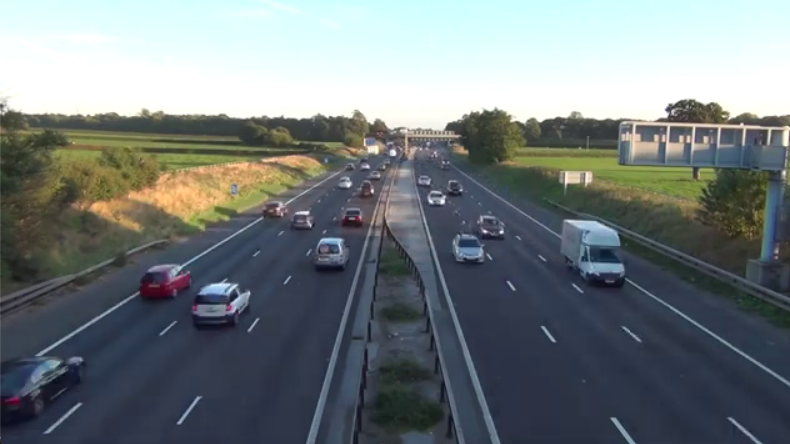
\includegraphics[width = 10cm]{ImagenesLatex/im1.png}{}
    \caption{Imagen descriptiva del vídeo}
    \label{fig:enter-label}
\end{figure}
Ahora se detecta cada coche con una cierta precisión.
\begin{figure}[h!]
    \centering
    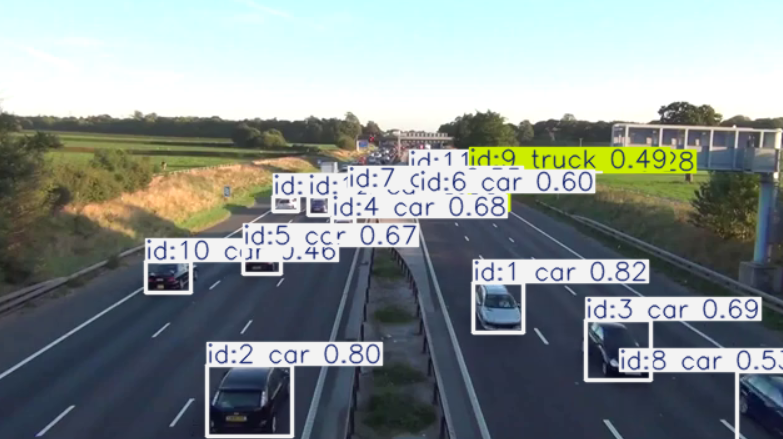
\includegraphics[width = 10cm]{ImagenesLatex/im2.png}{}
    \caption{Identificadores y Precisión de cada Vehículo}
    \label{fig:enter-label}
\end{figure}
En el siguiente frame se cuenta el número de vehículos en un ROI concreto.
\begin{figure}[h!]
    \centering
    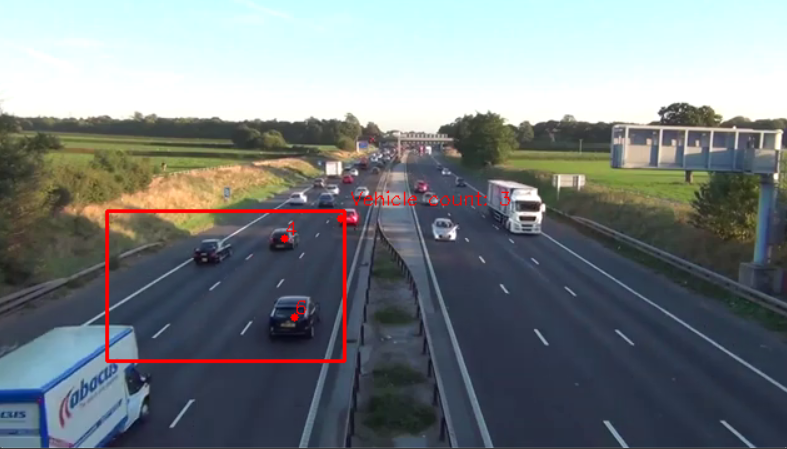
\includegraphics[width = 10cm]{ImagenesLatex/im3.png}{}
    \caption{Contador vehículos en ROI}
    \label{fig:enter-label}
\end{figure}
En el próximo frame se calcula la velocidad en píxeles por segundo de cada vehículo que esté dentro de la ROI.
\begin{figure}[h!]
    \centering
    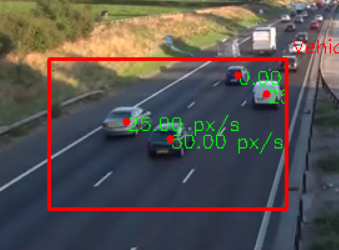
\includegraphics[width = 10cm]{ImagenesLatex/im4.png}{}
    \caption{Velocidad vehículos}
    \label{fig:enter-label}
\end{figure}

\subsection{Evaluación y Validación del Sistema}
Para evaluar el modelo se han hecho dos pruebas: de precisión - se compararon las detecciones realizadas con YOLO con observaciones manuales para evaluar qué tan bien se identificaron los vehículos -, y validación de velocidades para ver si son coherentes y así ajustarlos.

\subsection{Otras Consideraciones}
Este proyecto sienta las bases para futuras implementaciones más avanzadas como puede ser la conversión de las velocidades de píxeles por frame a km/h calibrando el sistema con distancias reales. Se podría usar en aplicaciones como análisis de tráfico en tiempo real o monitoreo de carreteras para estudios de seguridad en las carreteras.


% Fuente
Dataset: el vídeo se encuentra en el enlace siguiente:
$"https://www.youtube.com/watch?v=wqctLW0Hb_0"$



\subsection{Exploración del dataset}
Para esta práctica se ha elegido un vídeo en vista aérea de coches que van circulando por una autopista en dos sentidos contrarios.  Este dura unos 34 minutos y tiene una resolución de 640x360 píxeles.
El vídeo tiene buena iluminación, contraste y claridad.


